\subsection{Long-Term Temporal Structure}
\begin{frame}{Long-Term Temporal Structure}
    Understanding complex actions in videos often requires analyzing long-term temporal structure, rather than relying solely on short clips. This involves capturing dependencies and patterns that span extended periods, which are crucial for recognizing actions composed of multiple stages or events.

    \begin{itemize}
        \item \textbf{Temporal Segmentation:} Divides a video into meaningful segments based on changes in activity.
        \item \textbf{Temporal Action Proposals:} Identifies candidate time intervals where actions may occur.
    \end{itemize}

    These techniques enable models to focus on relevant portions of the video and improve the recognition of complex, long-duration actions.
\end{frame}

\begin{frame}{Modelling Long-Term Structure}
    Several approaches have been developed to effectively model long-term temporal dependencies in videos:

    \begin{itemize}
        \item \textbf{Hierarchical RNNs and LSTMs:} Stack multiple recurrent layers to capture both short-term and long-term dependencies at different temporal scales.
        \item \textbf{Temporal Segment Networks (TSN):} Sample frames or segments sparsely across the entire video and aggregate their representations to model long-range structure.
        \item \textbf{Memory Networks:} Utilize external memory modules to store and retrieve information across hundreds of frames, enabling reasoning over extended temporal contexts.
    \end{itemize}

    These methods help in recognizing actions that unfold over long durations and involve multiple stages.
\end{frame}

\begin{frame}{Modelling Long-Term Structure}
    \begin{itemize}
        \item So far, all our temporal CNNs only model local motion between frames in very short clips of approximately 2--5 seconds.
        \item What about long-term structure?
        \item<2-> \textbf{We know how to handle sequences!}
        \item<2-> How about \textbf{recurrent networks}?
    \end{itemize}
    \begin{figure}
        \centering
        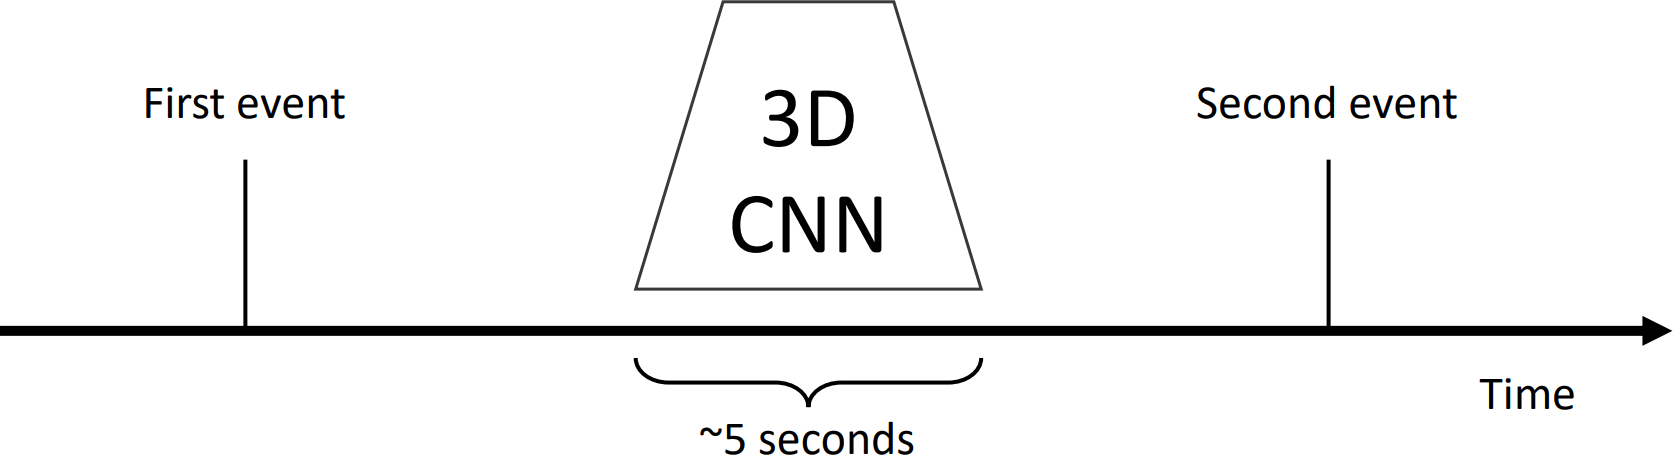
\includegraphics[width=1\textwidth,height=0.5\textheight,keepaspectratio]{images/video/slide_25_1_img.png}
    \end{figure}
\end{frame}

\begin{frame}{Modelling Long-Term Structure}
    \begin{itemize}
        \item Process local features using recurrent network (e.g. LSTM)
        \item Many to many: one output per video frame
    \end{itemize}
    \begin{figure}
        \centering
        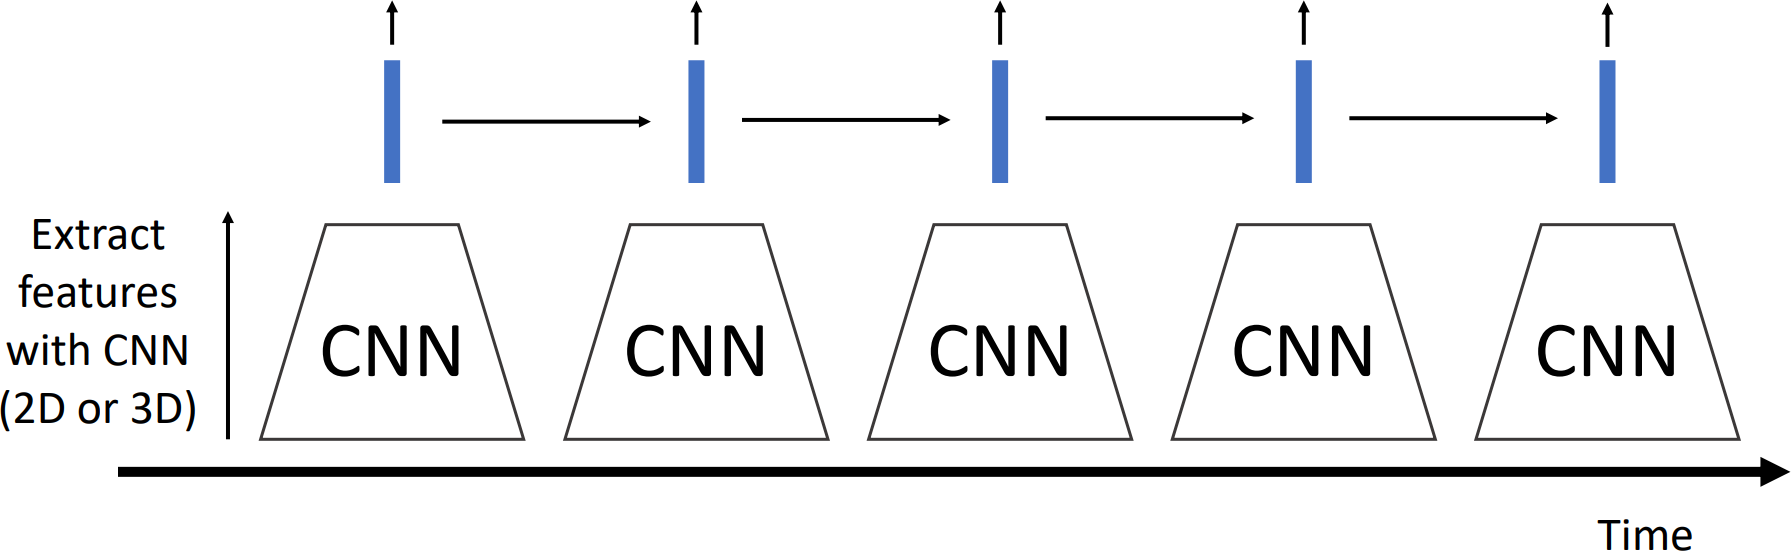
\includegraphics[width=1\textwidth,height=0.5\textheight,keepaspectratio]{images/video/slide_27_1_img.png}
    \end{figure}
\end{frame}

\begin{frame}[allowframebreaks]{Recurrent Convolutional Network}
    \begin{figure}
        \centering
        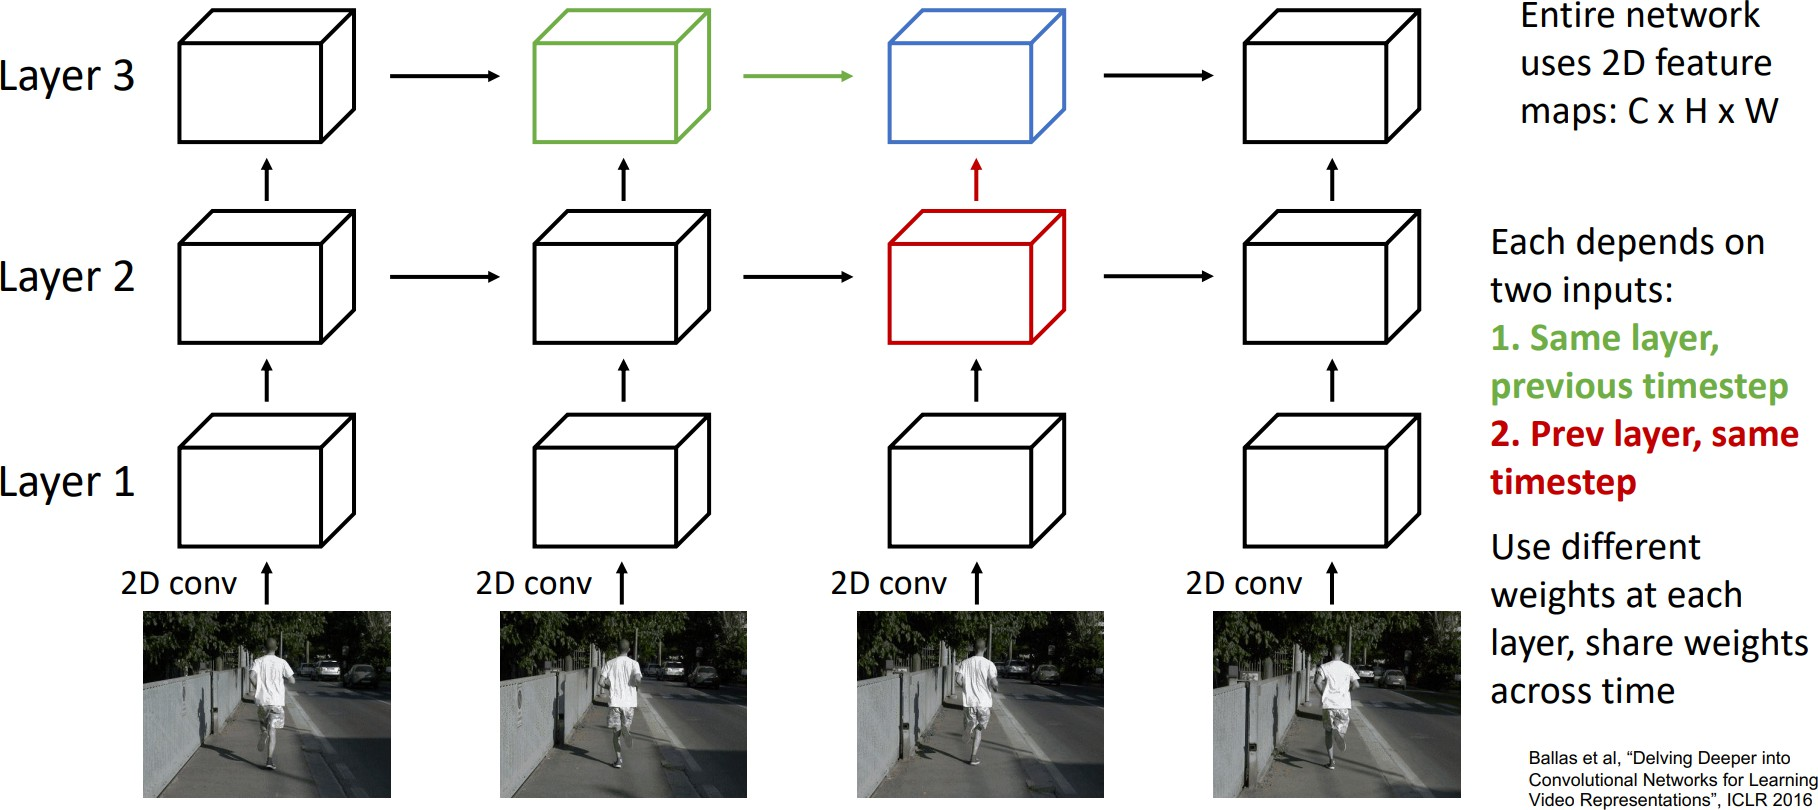
\includegraphics[width=1\textwidth,height=0.9\textheight,keepaspectratio]{images/video/slide_28_1_img.jpg}
    \end{figure}
\framebreak
    \begin{figure}
        \centering
        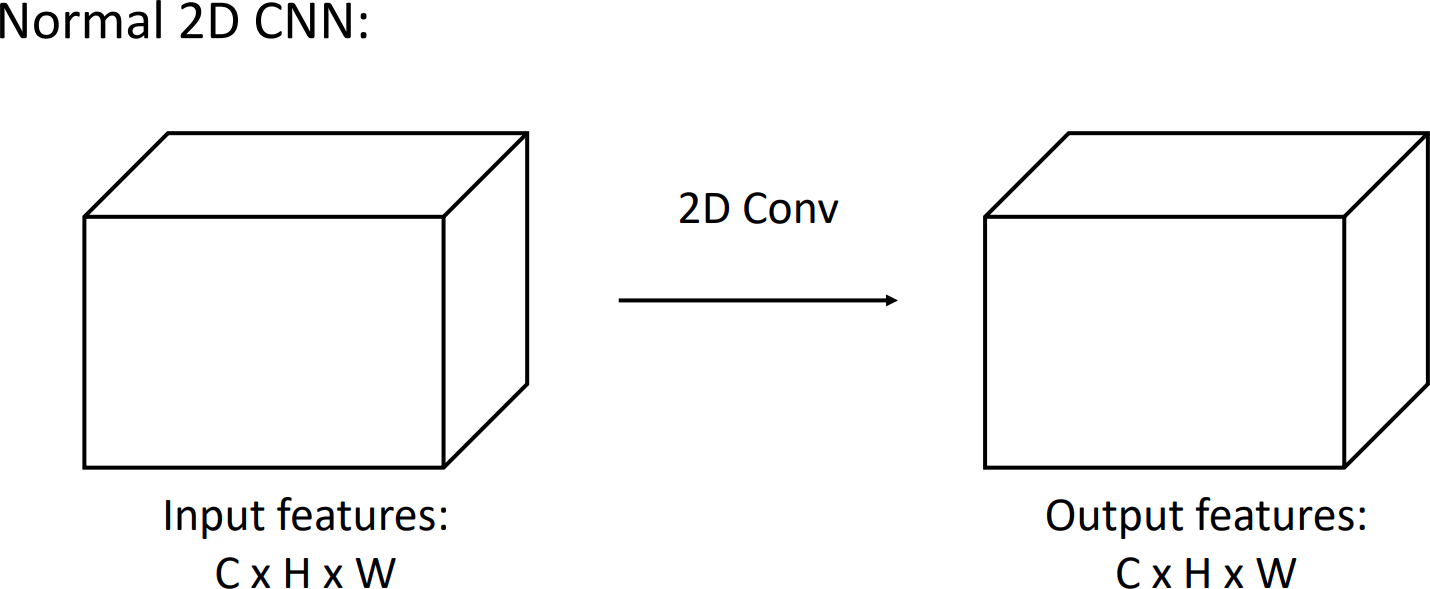
\includegraphics[width=1\textwidth,height=0.9\textheight,keepaspectratio]{images/video/slide_29_1_img.png}
    \end{figure}
\framebreak
    \begin{figure}
        \centering
        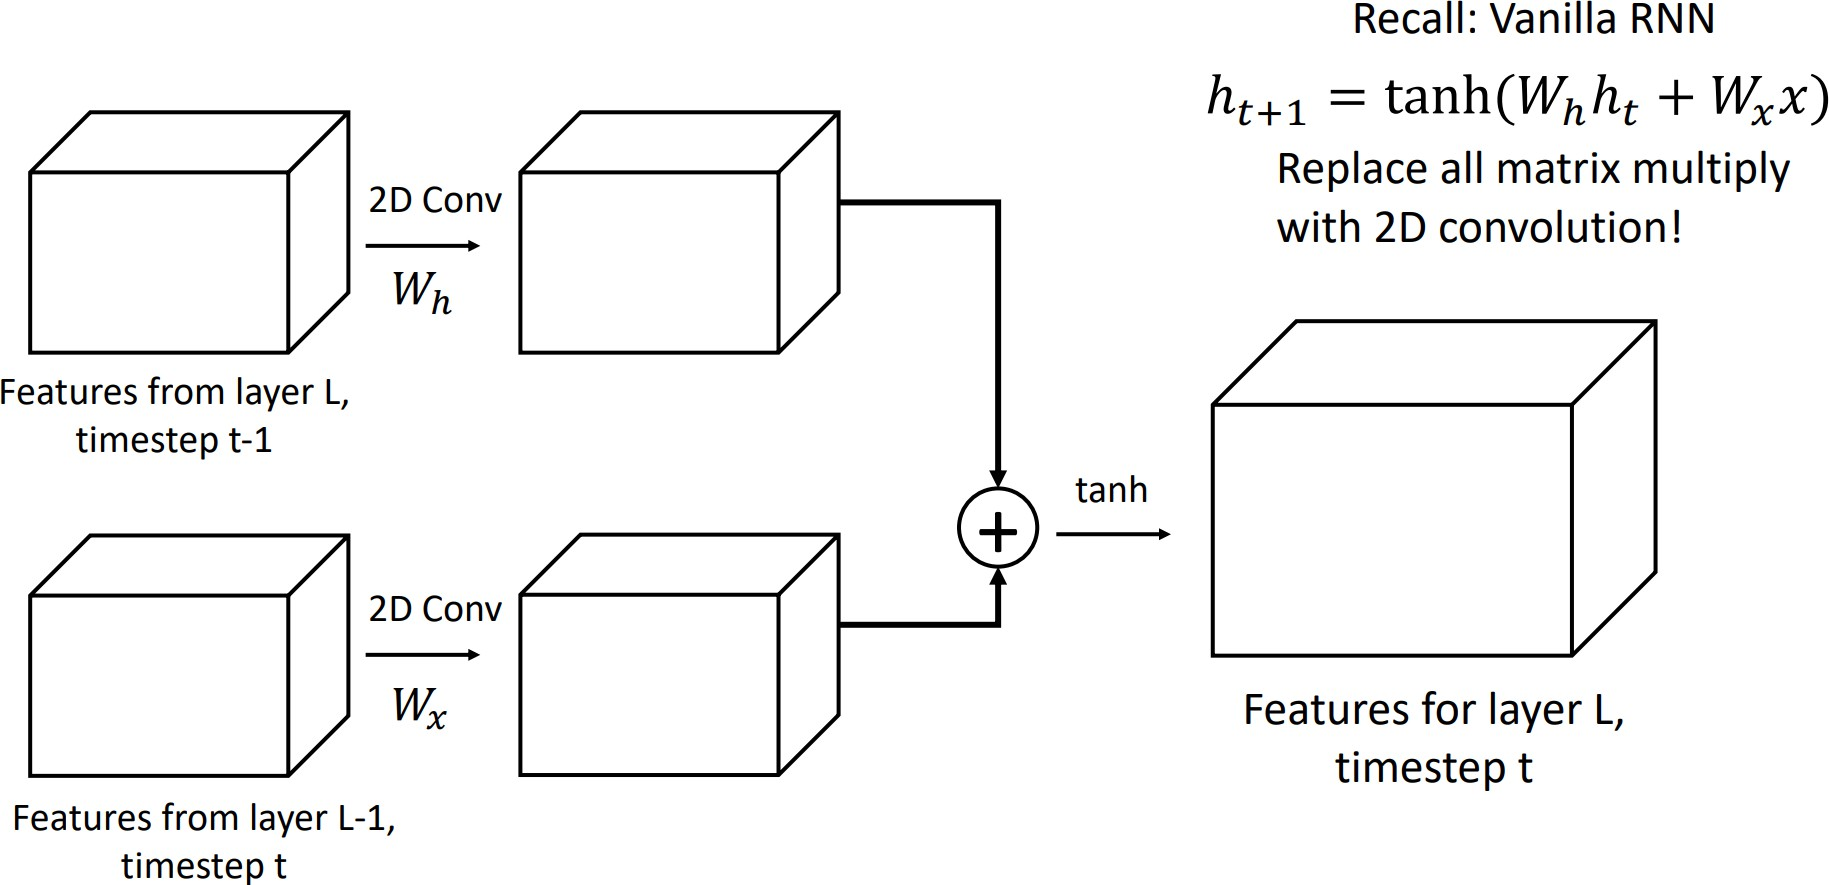
\includegraphics[width=1\textwidth,height=0.9\textheight,keepaspectratio]{images/video/slide_30_1_img.jpg}
    \end{figure}
\end{frame}

\begin{frame}[allowframebreaks]{Modeling long-term temporal structure}
    \begin{figure}
        \centering
        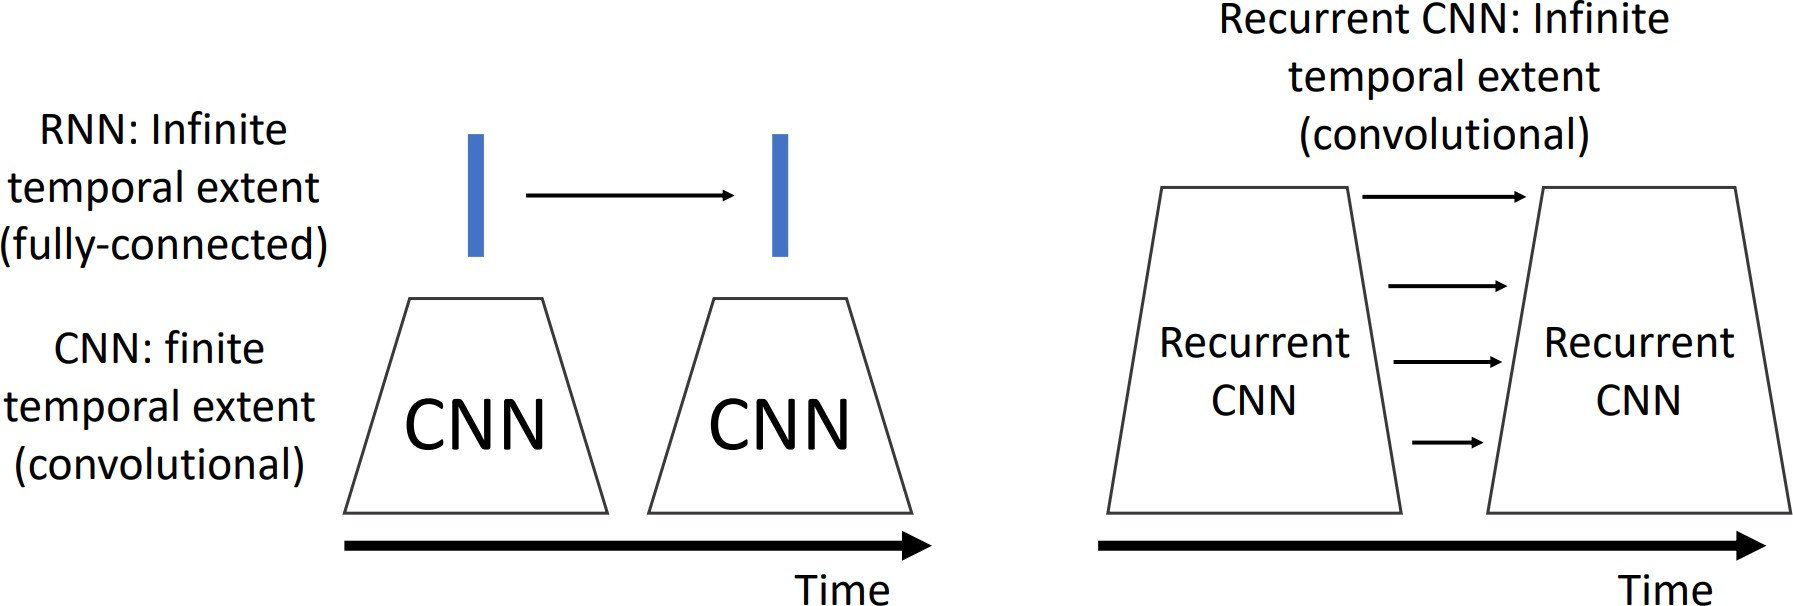
\includegraphics[width=1\textwidth,height=0.9\textheight,keepaspectratio]{images/video/slide_31_1_img.jpg}
    \end{figure}
\framebreak
    \begin{figure}
        \centering
        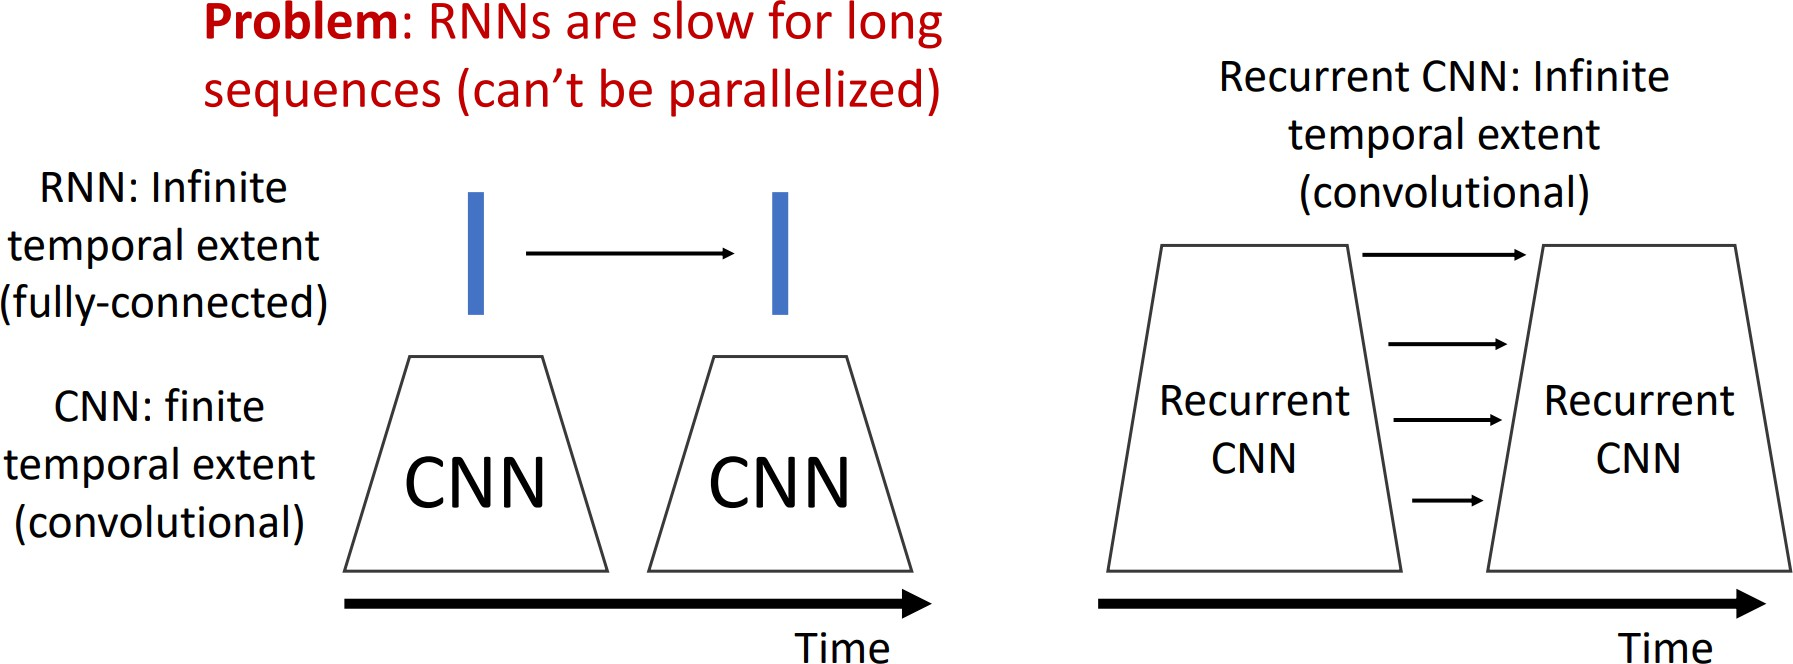
\includegraphics[width=1\textwidth,height=0.9\textheight,keepaspectratio]{images/video/slide_32_1_img.jpg}
    \end{figure}
\end{frame}